\section{Study 1: One Strategy, Three Markets}
\label{sec:study1}

\subsection{Design}

The control is a JMA(7)/JMA(21) crossover whose parameters are walk-forward selected from a small grid. It exits with
a fixed $\SoneSl\times$ATR stop and $\SoneTp\times$ATR target in forex, and with a $\SoneSl\times$ATR stop and a
ratcheting trailing stop in commodities and Indian equities. The three markets are a four-pair forex sleeve (AUDNZD,
CADJPY, AUDUSD, NZDUSD), five commodities (WTI and Brent crude, natural gas, gold, silver), and 48 NIFTY-50 stocks
with an annual sector-curation overlay. Each market's models were frozen at 70\% of its calendar span. Results are
reported on a \emph{holdout} window after the freeze and, for commodities and Indian equities, on a \emph{forward}
window of data collected after the study was designed (Fig.~\ref{fig:timeline}).

Study~1 keeps the statistical conventions of the original study, which Appendix~\ref{app:s1stats} states in full:
each trade stream becomes a daily series by averaging the returns of the trades exiting each day, Sharpe ratios are
annualized with a 6\% per-year risk-free rate, and a configuration is called significant iff the 95\% confidence
interval (CI) of the per-day Sharpe difference, from 2{,}000 unpaired i.i.d.\ bootstrap resamples, excludes zero.
The grid comprises five components, four combinations, three markets, and up to two windows, for \SoneConfigs{}
configurations in total.

\subsection{Results}

Across the \SoneConfigs{} configurations, \SoneSigGain{} show a significant improvement and \SoneSigLoss{} a
significant loss (Figs.~\ref{fig:s1matrix} and~\ref{fig:s1forest}). ML exit is the clearest failure: it loses
significantly in \SoneExitSigLoss{} of its \SoneExitConfigs{} configurations and inflates the trade count by a factor
of \SoneExitInflLo--\SoneExitInflHi, because a per-bar continuation classifier exits early and releases crossovers that
a longer-held rule-based trade would have absorbed. On the original forex data, where the control's holdout Sharpe
ratio is \SoneForexBase{}, \SoneForexSigLoss{} of \SoneForexConfigs{} configurations lose significantly. The closest
call is meta-labeling followed by position sizing in Indian equities: the holdout Sharpe ratio rises from
\SoneBestHoldBase{} to \SoneBestHoldVar{} (per-day CI $[\SoneBestHoldCiLo, \SoneBestHoldCiHi]$, approximately
$[\SoneBestHoldCiLoAnn, \SoneBestHoldCiHiAnn]$ annualized) and the forward Sharpe ratio from \SoneBestFwdBase{} to
\SoneBestFwdVar{} (CI $[\SoneBestFwdCiLo, \SoneBestFwdCiHi]$); neither change is significant. Every per-configuration
value is provided as supplementary data (see the Data and Code Availability section).

\begin{figure*}[!t]
\centering
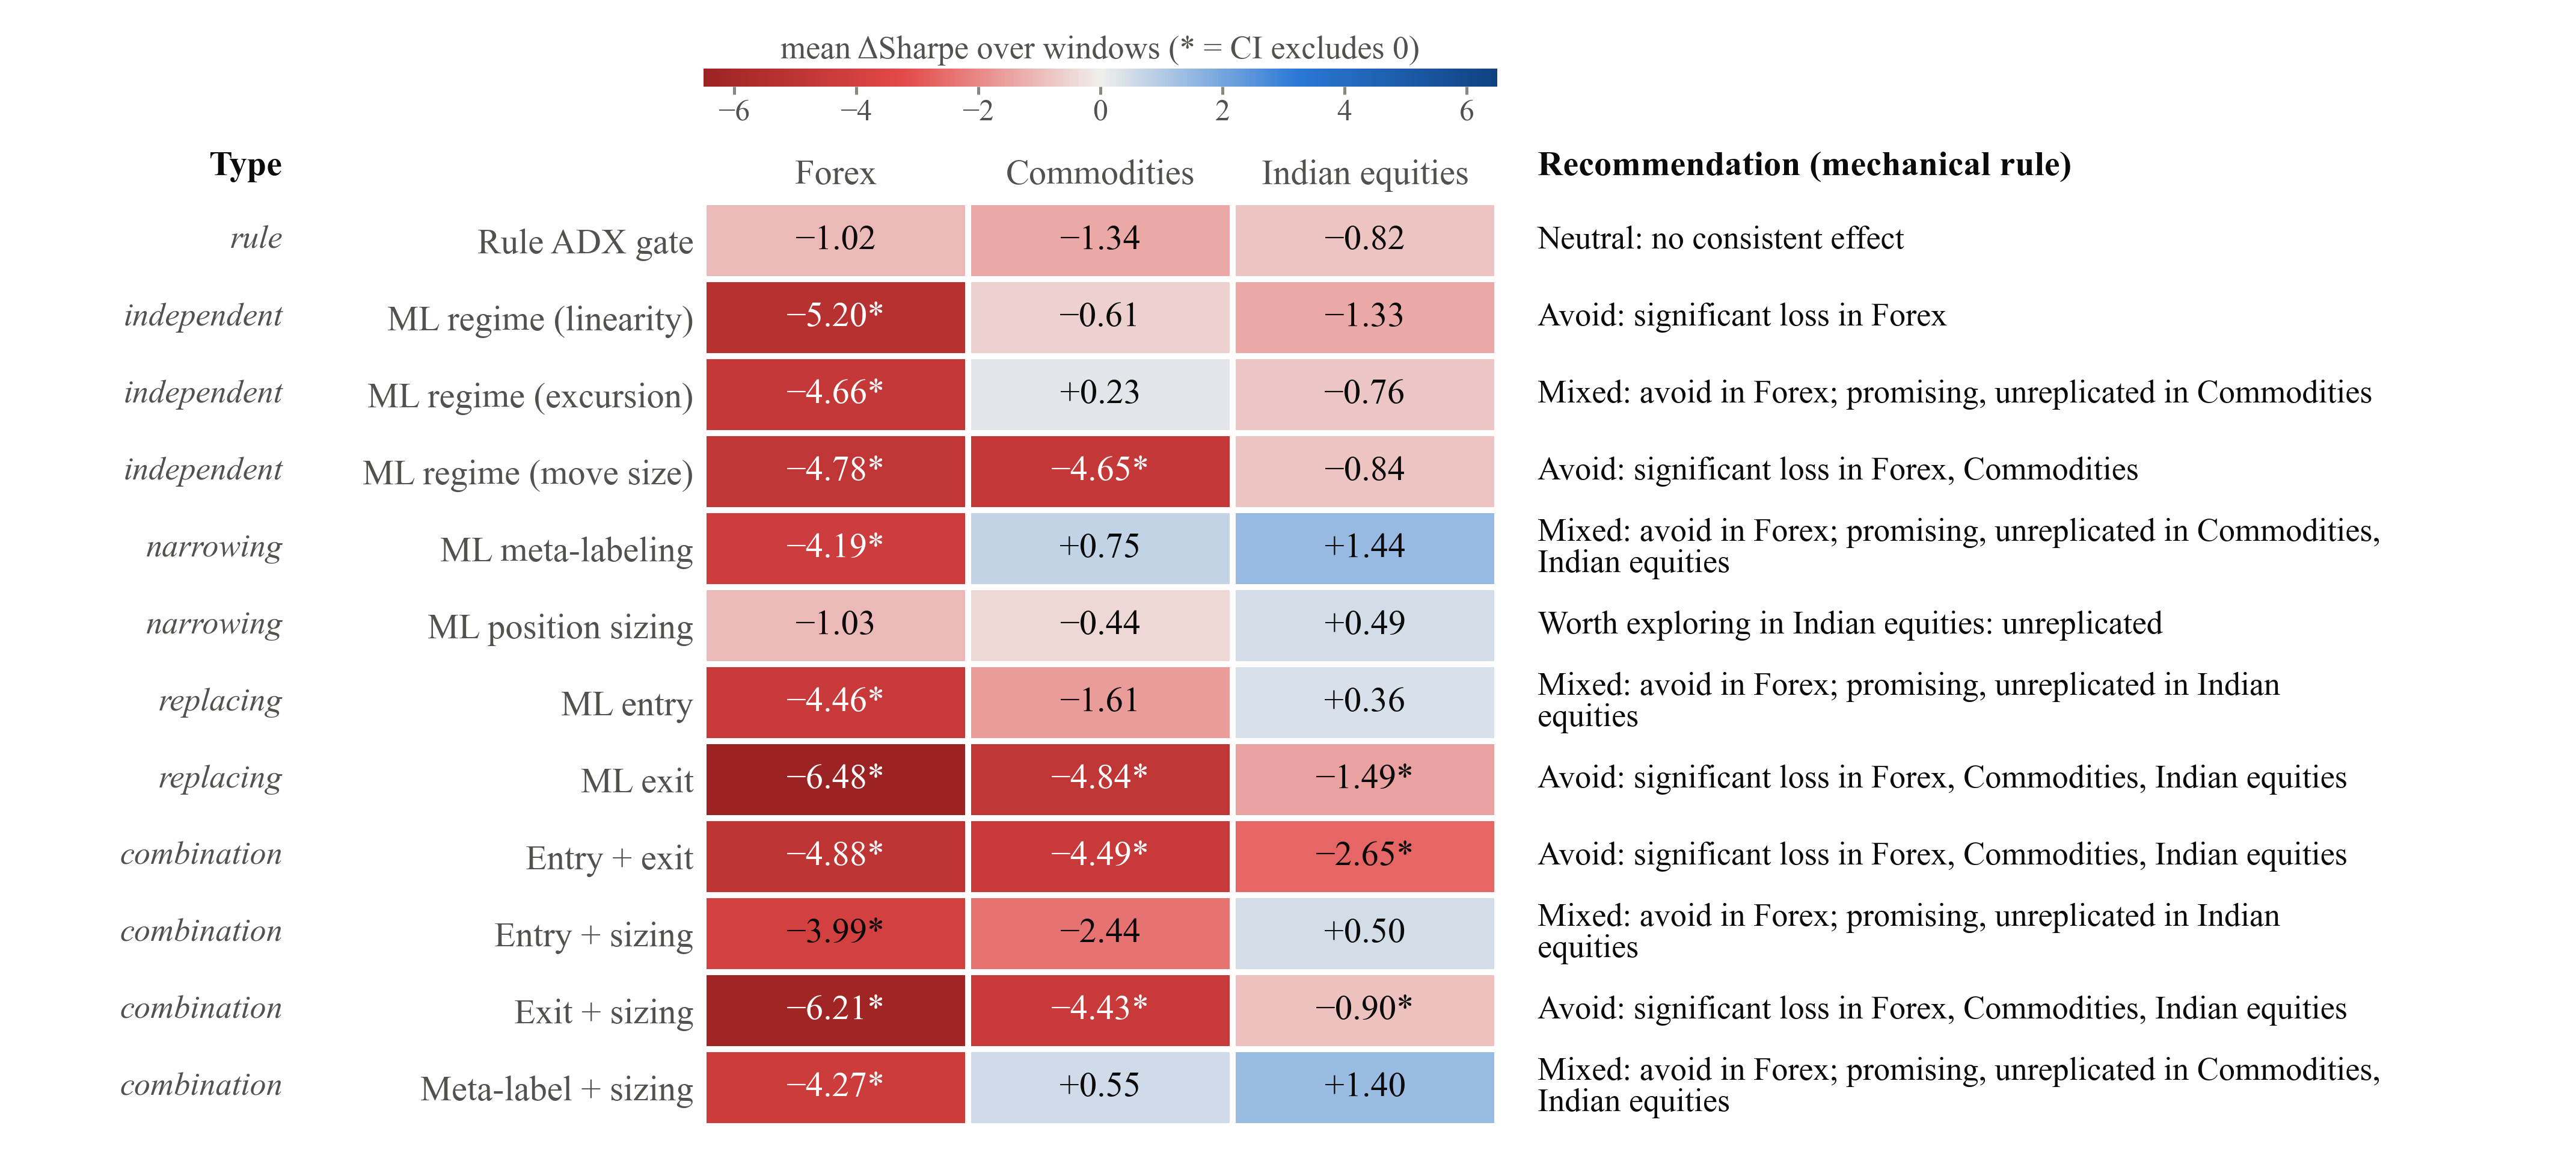
\includegraphics[width=7.14in]{figures/s1_matrix.png}
\caption{Study~1 opportunity matrix: mean $\Delta$Sharpe over windows for each component and market (* = CI excludes
zero in at least one window), with the taxonomy type and the recommendation produced by the mechanical rule of the
original study.}
\label{fig:s1matrix}
\end{figure*}

\begin{figure*}[!t]
\centering
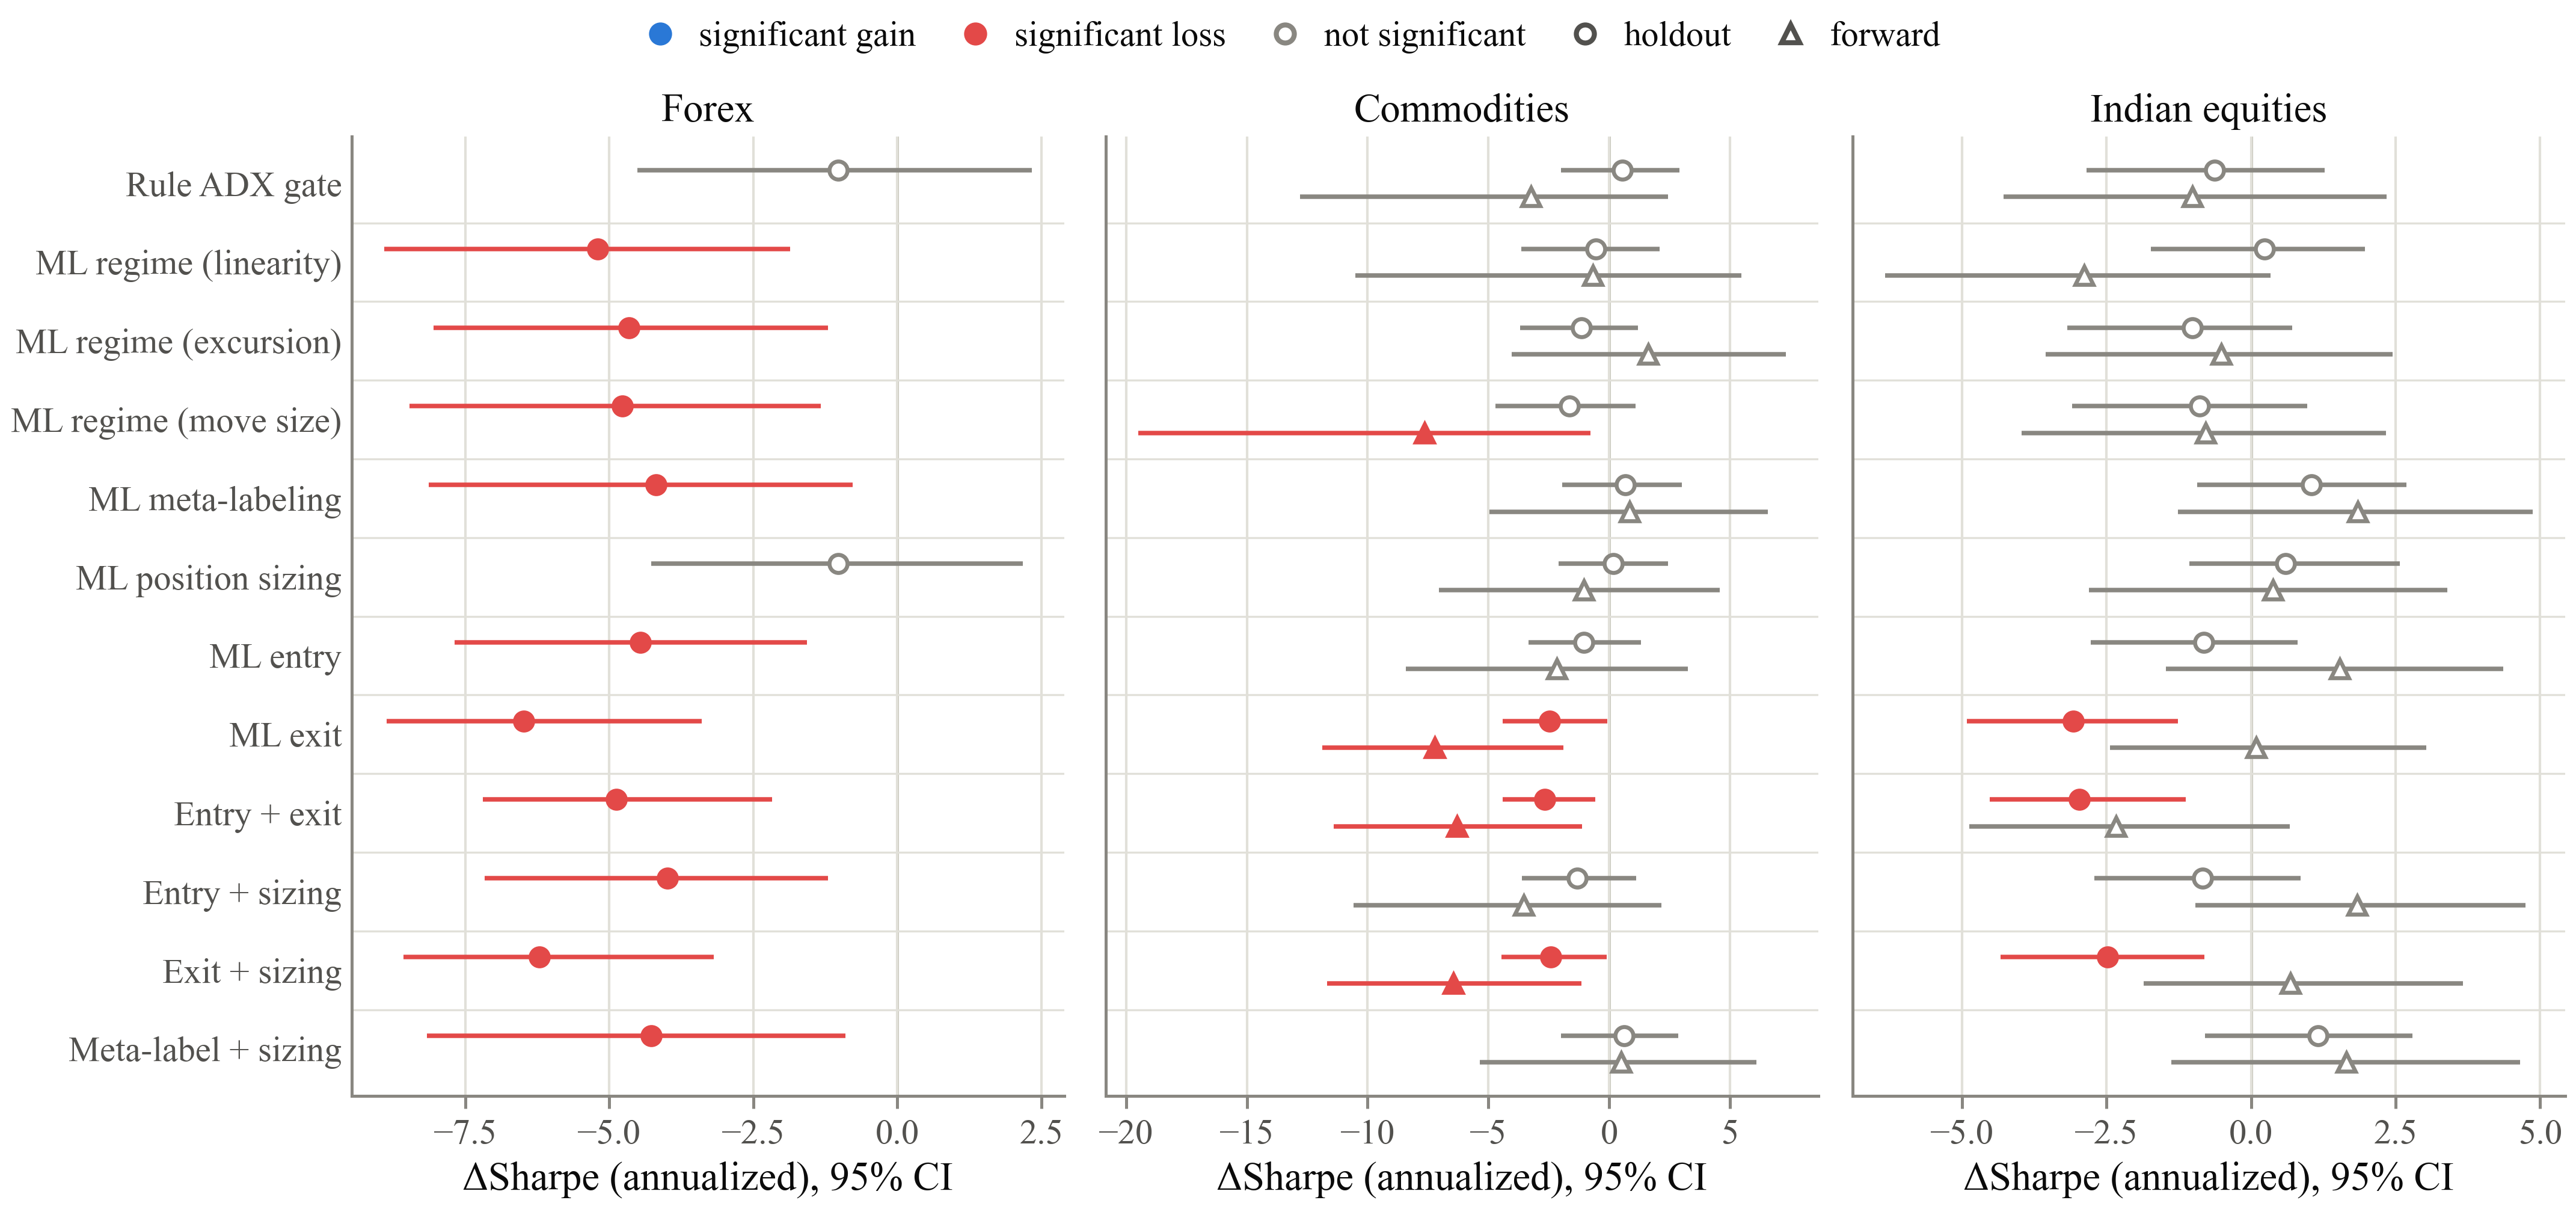
\includegraphics[width=7.14in]{figures/s1_forest.png}
\caption{Every Study~1 configuration. Markers show the annualized $\Delta$Sharpe (circles: holdout; triangles:
forward) and bars the bootstrap CI rescaled by $\sqrt{252}$ so that both share one axis. Filled markers are
significant; the forex market has no forward window.}
\label{fig:s1forest}
\end{figure*}

\subsection{Independent Re-Implementation}

The released package re-implements Study~1 from scratch (Appendix~\ref{app:repro}). Running it on the bundled data is
an independent replication with three known differences: a different forex data vendor with a flat 7\,bps cost, no
sector-curation overlay, and a single walk-forward over the full history. Fig.~\ref{fig:s1rep} compares the two
configuration by configuration. The re-implementation reproduces the headline: \SoneRepSigGain{} significant gains,
ML exit significantly harmful in every market with the trade count inflated by
\SoneRepExitInflLo--\SoneRepExitInflHi, and \SoneRepSignAgree{} of \SoneRepN{} configurations agreeing in sign. It
does not reproduce the market-level claims. With different forex data (control Sharpe \SoneRepForexBase{}), only
\SoneRepForexSigLoss{} forex configurations lose significantly, and meta-labeling flips from \SoneMetaForexPaper{} to
\SoneMetaForexRep{}. The meta-label + sizing near-miss replicates on the forward window (\SoneBestFwdDelta{} vs.\
\SoneRepBestFwd{}) but not on the holdout (\SoneBestHoldDelta{} vs.\ \SoneRepBestHold{}), where the control itself
rises to \SoneRepIndiaBase{} without curation.

\begin{figure}[!t]
\centering
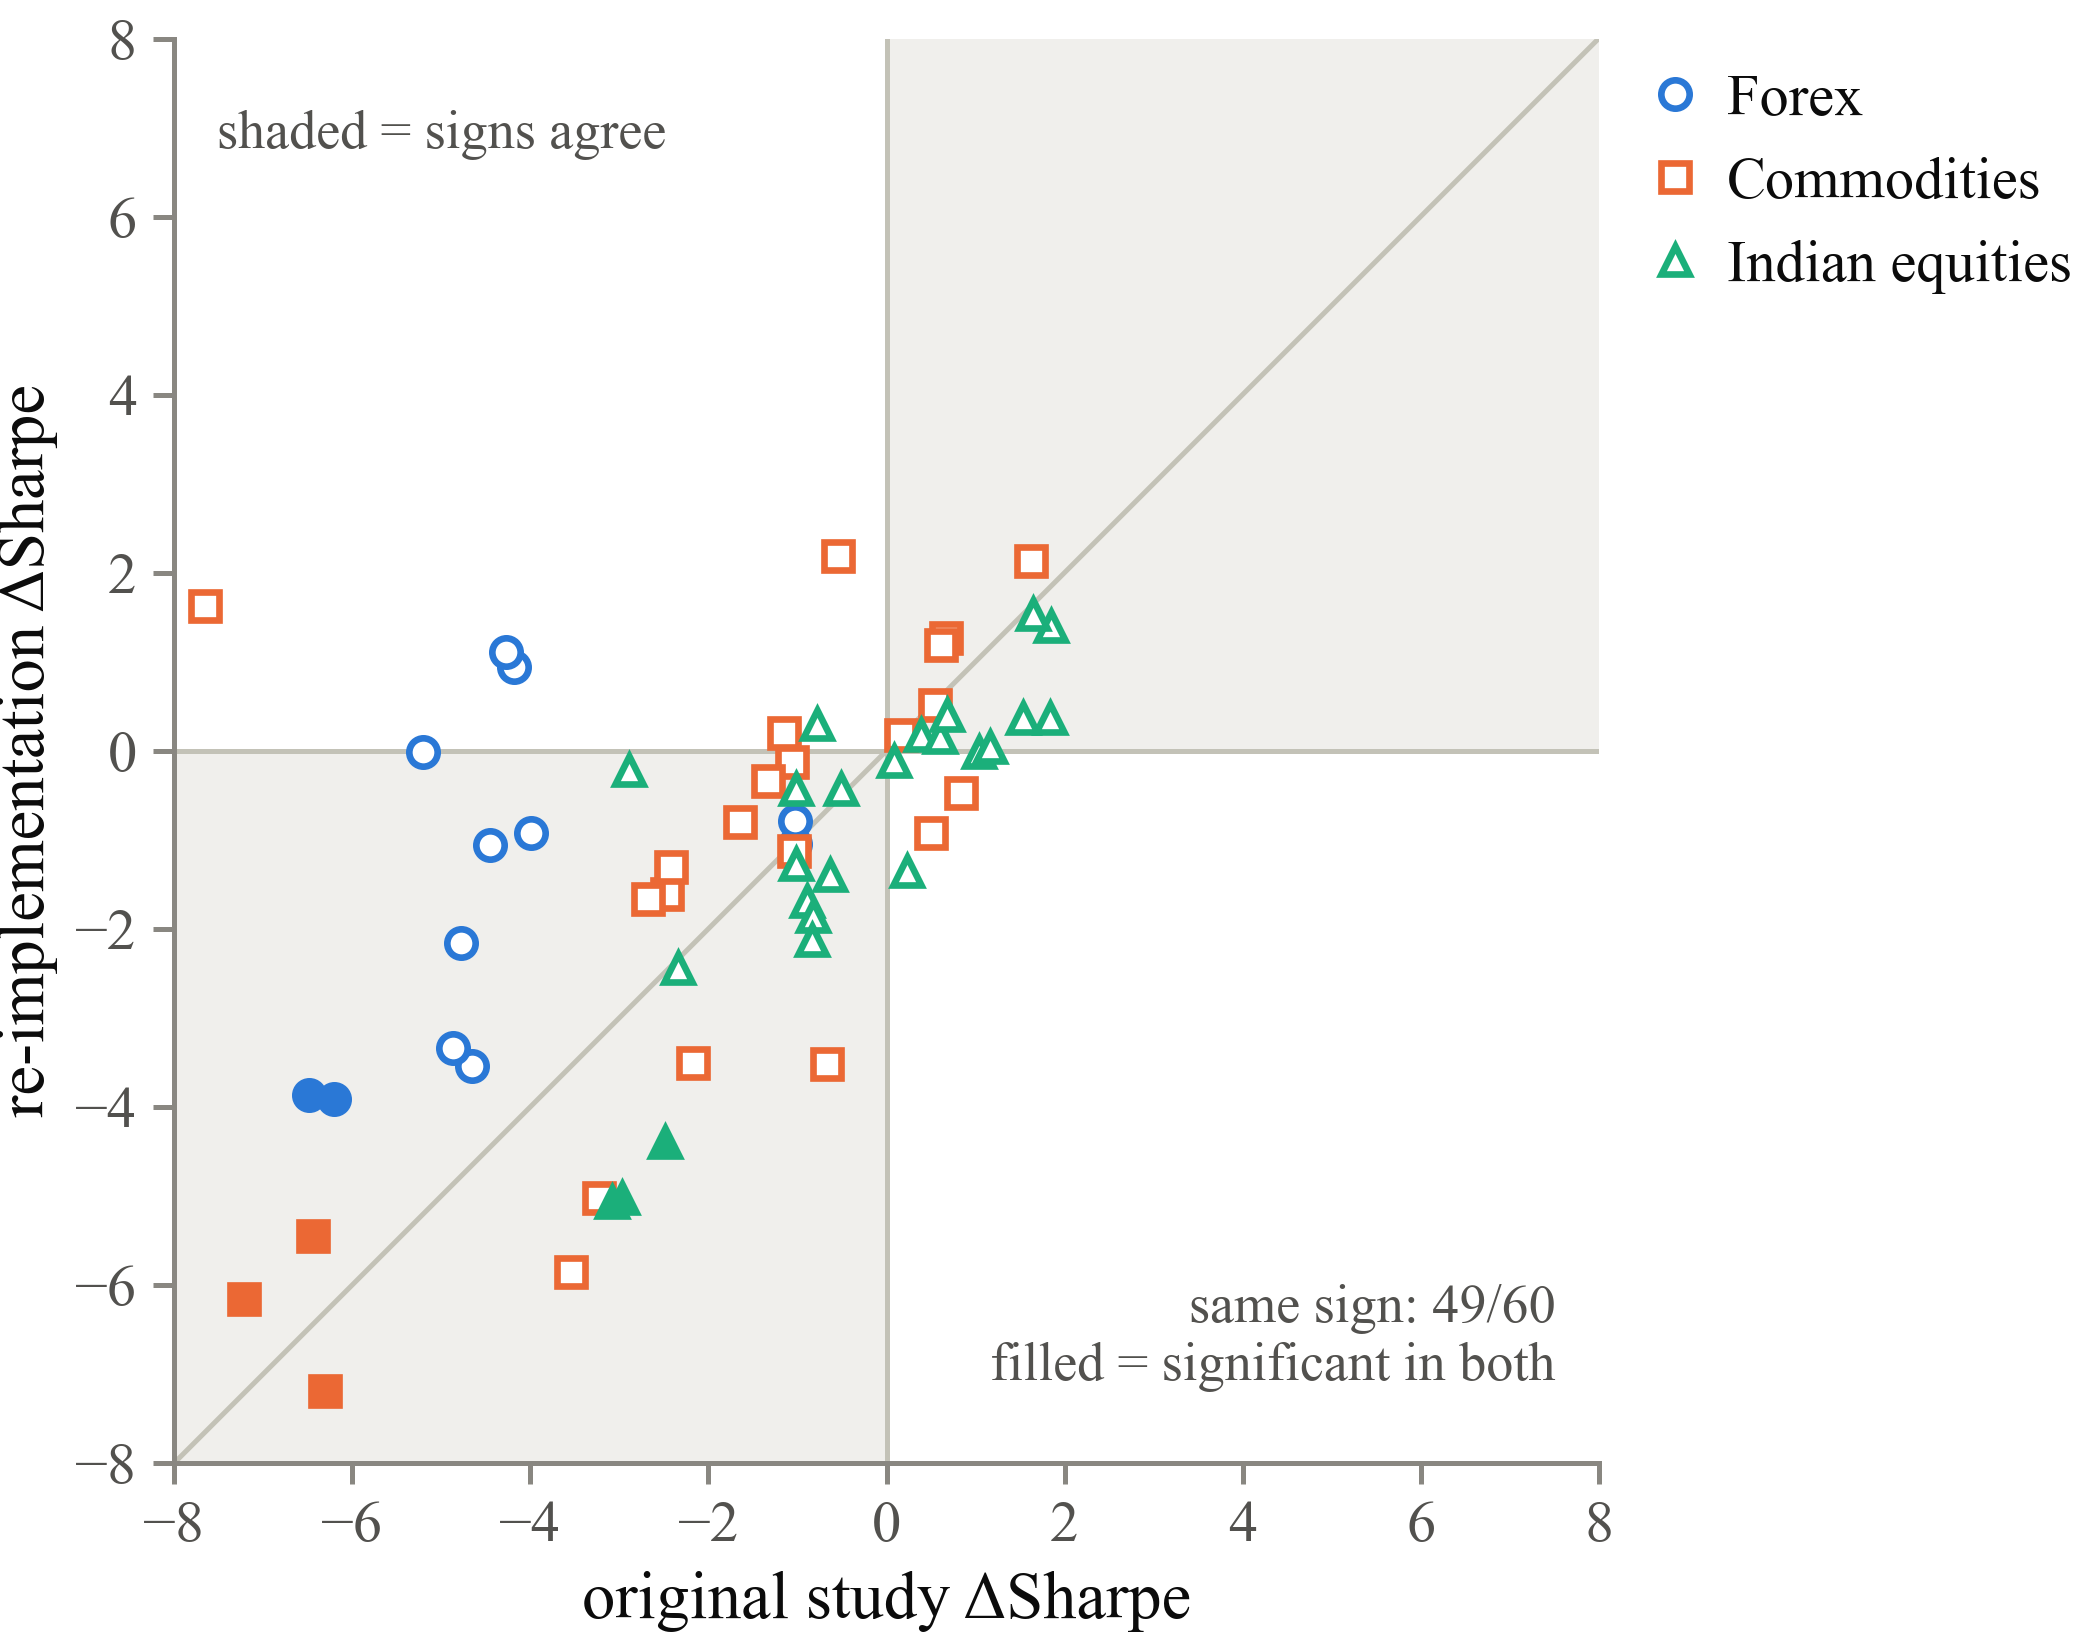
\includegraphics[width=3.487in]{figures/s1_replication.png}
\caption{Study~1: original $\Delta$Sharpe against the independent re-implementation, one point per configuration.
Shaded quadrants mark sign agreement; filled markers are significant in both.}
\label{fig:s1rep}
\end{figure}

\subsection{Open Questions}

Study~1 therefore leaves three questions open, which Study~2 was pre-registered to answer. Does the pattern hold for
other historically successful strategies, not only a JMA crossover? Does it hold across a much broader and more
diverse universe? And does it survive a second, independent freeze date, stricter execution assumptions, and a test
that respects the pairing and serial dependence of returns?
